\section{Describing dynamic behaviour with SDMs}
\subsection{LinkedList}
\label{sec:LinkedList}
As example to show you some main features, we use a simple LinkedList. As an experienced programmer you will know what a LinkedList is. But for a short summarize a LinkedList consists of nodes which have a \texttt{next} and a \texttt{previous} node (Fig.~\ref{linkedList}). As functions in this tutorial we have the possibility to insert a new Node before and after a node. A function to delete nodes exists too.

\begin{figure}[htbp]
	\centering
  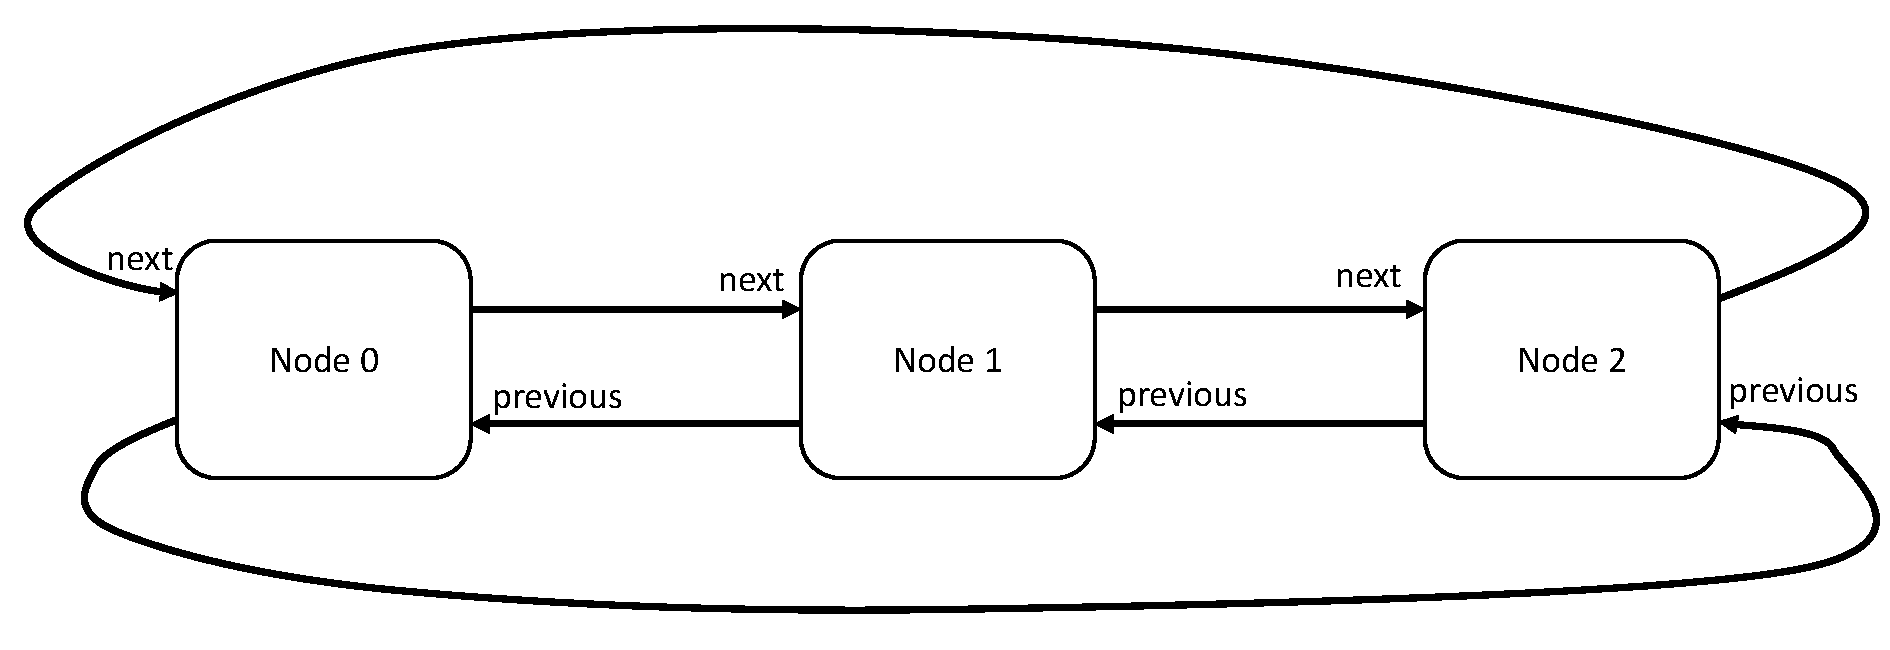
\includegraphics[width=1\textwidth]{LinkedList.pdf}
	\caption{Structure of a LinkedList} 
	\label{linkedList} 
\end{figure}

\subsection{Implementation of the LinkedList}
Now, after you remember what a LinkedList is, we inspect a possible implementation of it with the Moflon tool.

\begin{itemize}
\item First open the \texttt{org.moflon.demo.eap} file by double clicking on it. Now Enterprise Architect (EA) should open.

\item On the right side you see the \texttt{Project Browser} where you can see all projects. Expand the \texttt{org.moflon.demo} project an its package. Here are all classes listed. Also a classdiagram named \texttt{org.\-moflon.\-demo.\-double\-linked\-list} exists (Fig.~\ref{ea:overview}).


\item Open the classdiagram. Here you can see the necessary classes and their methods and parameters (Fig.~\ref{ea:classdiagram}).
\end{itemize}

The \texttt{List} class represents the LinkedList and contains \texttt{Node} classes as elements. As mentioned in section \ref{linkedList} each node contains a \texttt{next} and a \texttt{previous} node. To insert new nodes or to delete nodes there are three methods in \texttt{Node}.
\newline
As next step we will examine one method.

\begin{figure}[htbp]
	\centering
  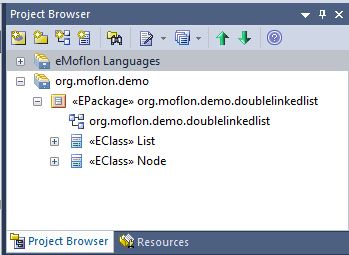
\includegraphics[width=0.5\textwidth]{ea_overview}
	\caption{EA Project Browser} 
	\label{ea:overview} 
\end{figure}

\begin{figure}[htbp]
	\centering
  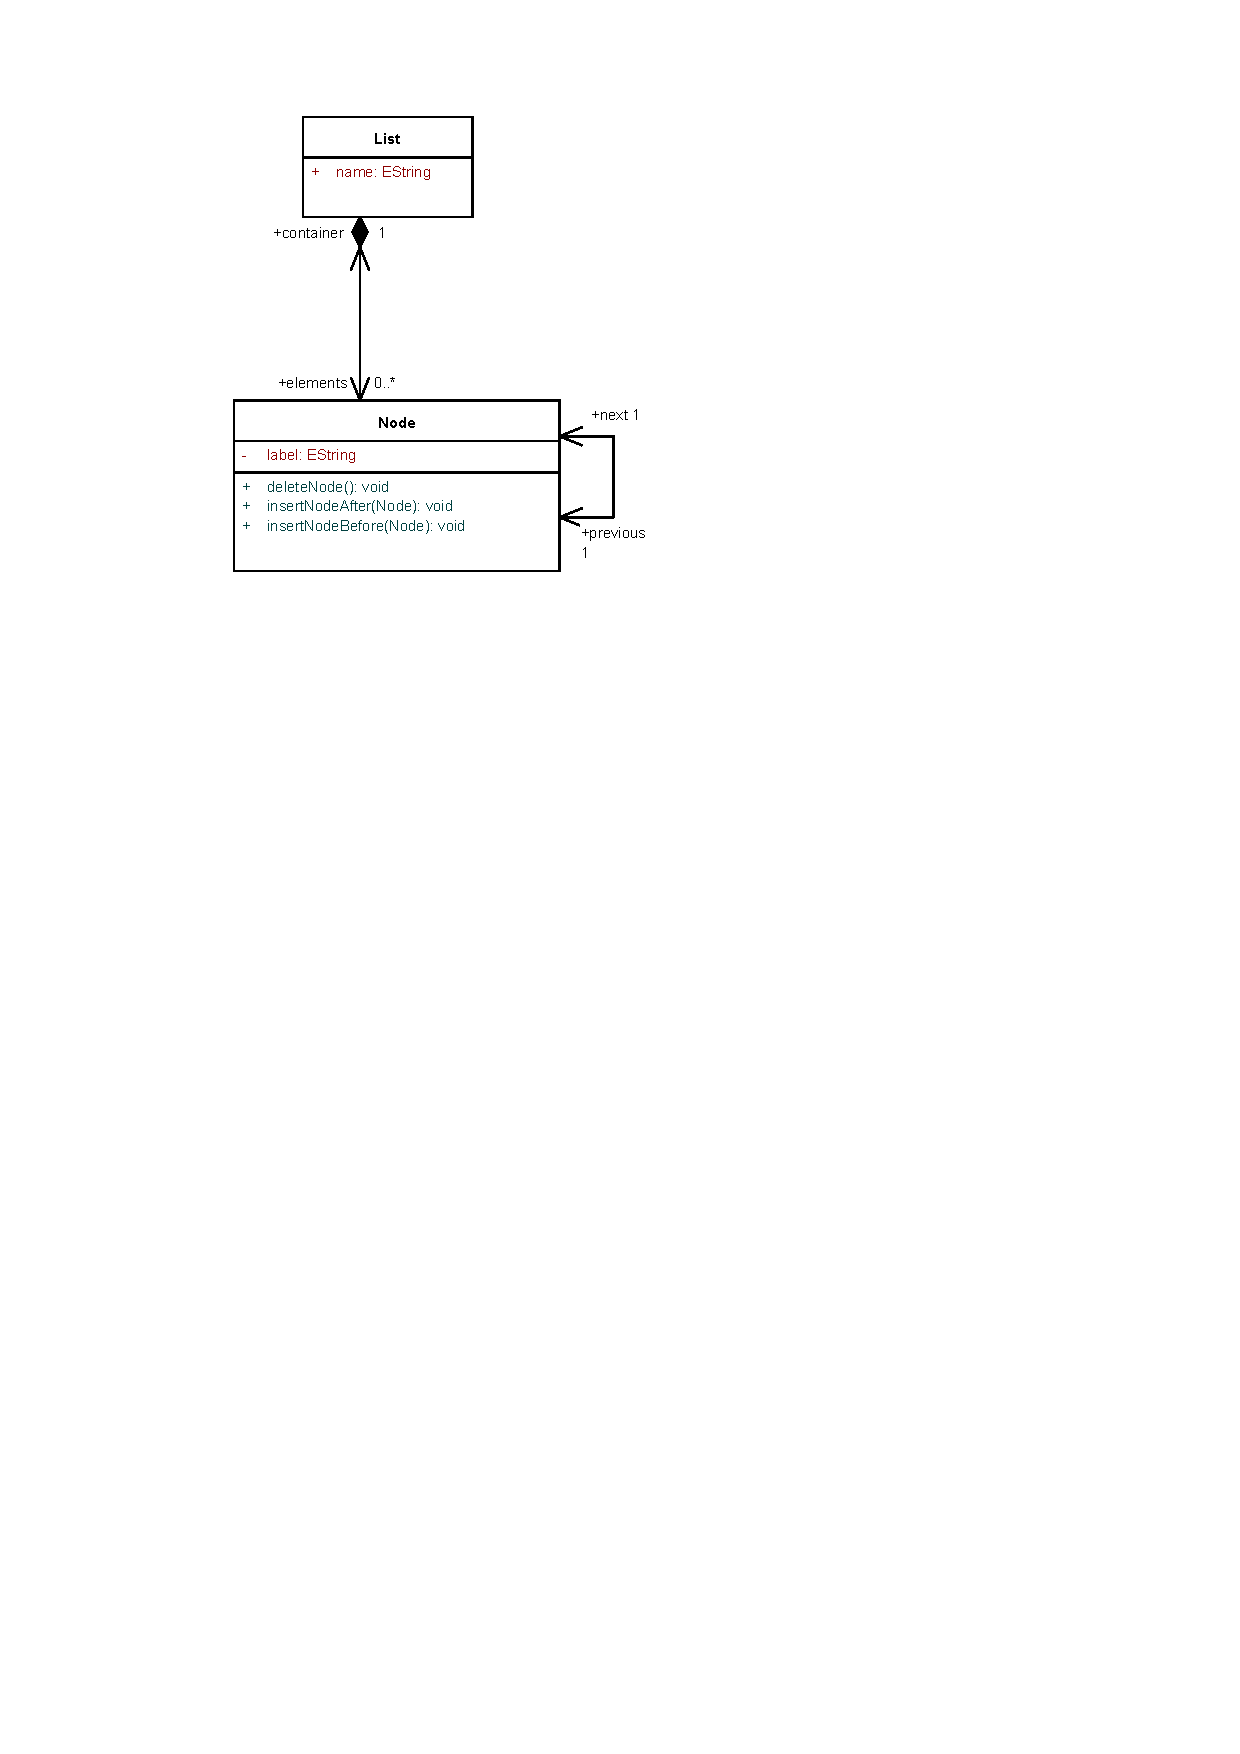
\includegraphics[width=0.6\textwidth]{ea_classdiagram}
	\caption{Classdiagram of the LinkedList} 
	\label{ea:classdiagram} 
\end{figure}





\subsection{The deleteNode Method}
Normally you would begin now tiping the code for the method implementation. But Moflon offers you the possibility to generate the code automatically by diagrams. We name these diagram types \texttt{Story Driven Modeling (SDM)}. These is a cool and easy way to describe method behaviours. But now lets see how this looks like.

\begin{itemize}
\item Open the \texttt{deleteNode Story Diagram} under \texttt{Node/deleteNode()} \newline (Fig.~\ref{open_deleteNode}).
\end{itemize}
\begin{figure}[htbp]
	\centering
  \includegraphics[width=0.44\textwidth]{ea_sdm_select_deleteNode}
	\caption{Open deleteNode Story Diagram} 
	\label{open_deleteNode} 
\end{figure}

In Fig.~\ref{sdm_deleteNode} you see the SDM which describes the whole function of the \texttt{deleteNode} method. A red element will be deleted in the method, a green one created. Black elements still consists. With this knowledge you can easily understand what is going on in this diagram.
\newline
In detail the next node of the present node will be destroied. This is marked by the red frame. The links to the next node will be destroied too. To get no leak in the list the next next node must set as the new next node to the present node. This link is marked as green, because it must be created. 
\newline
For further information please refer to Part III of the handbook. There is everything explained in detail. But here you can see to describe a whole method is really easy.

\begin{figure}[htbp]
	\centering
  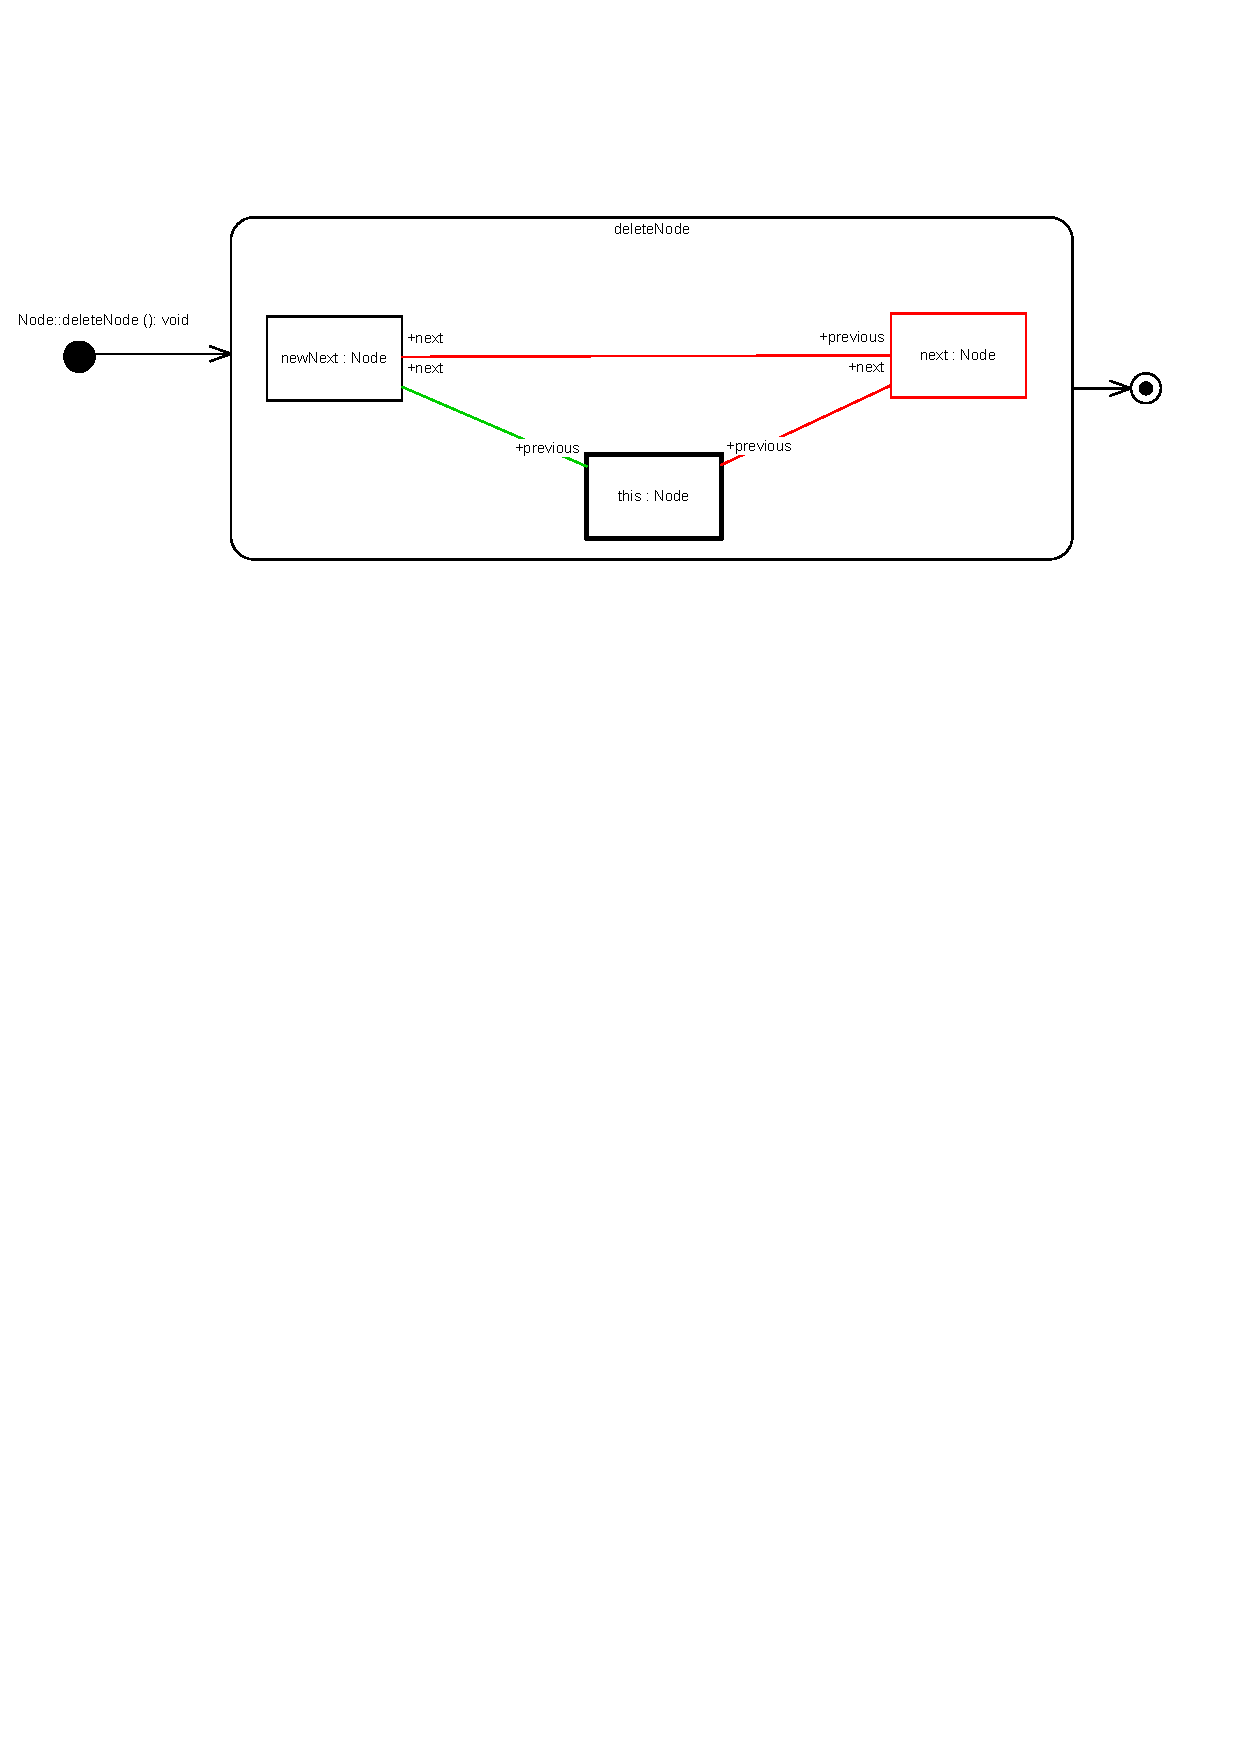
\includegraphics[width=1.2\textwidth]{ea_sdm_deleteNode}
	\caption{deleteNode SDM} 
	\label{sdm_deleteNode} 
\end{figure}



